\chapter{Introducción específica} % Main chapter title

\label{Chapter2}



%----------------------------------------------------------------------------------------
%	SECTION 1
%----------------------------------------------------------------------------------------
En este capítulo se presenta una breve introducción técnica a las herramientas de hardware y software utilizadas en el trabajo.

\section{Tecnologías de hardware y firmware utilizadas}


\subsection{Robot de exploración ambiental}

Como dispositivo físico en la capa de percepción, se utilizó el robot de exploración ambiental desarrollado en el marco de la carrera de Especialización de Sistemas Embebidos \citep{cese_gonzalo_memoria}. En la figura \ref{fig:Robot_y_Joystick_1} se puede apreciar una foto del mismo.


\begin{center}
   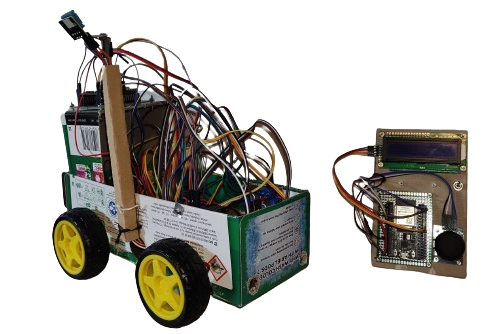
\includegraphics[scale=0.5]{Robot_y_Joystick_1}
   \captionof{figure}{Robot de exploración ambiental.}
   \label{fig:Robot_y_Joystick_1}
\end{center}

El robot de exploración ambiental es un sistema embebido desarrollado con el marco de desarrollo ESP-IDF \cite{ESPIDF_home} de \textit{Espressif Systems} que utiliza un microcontrolador ESP32 \cite{ESP32} y FreeRTOS \citep{FreeRTOS} como sistema operativo. Está diseñado para explorar terrenos mediante control de joystick y para obtener parámetros ambientales como luminosidad, presión atmosférica, temperatura y humedad.

\subsection{Microcontrolador ESP32}


ESP32 \cite{ESP32} es una serie de microcontroladores embebidos en un chip con Wi-Fi y Bluetooth integrados, de bajo costo y consumo, desarrollado por \textit{Espressif Systems}. Emplea dos cores Xtensa® 32-bit LX6 CPU, incluye interruptores de antena, amplificador de potencia, amplificador de recepción de bajo ruido, un co-procesador ULP (\textit{Ultra Low Power}), módulos de administración de energía y varios periféricos.


\subsection{Marco de trabajo ESP-IDF}

El marco de trabajo ESP-IDF de \textit{Espressif Systems} proporciona un conjunto de recursos para facilitar el desarrollo de \textit{firmware} para ESP32. Utiliza FreeRTOS como sistema operativo base y brinda varias utilidades de desarrollo y bibliotecas de código para poder acceder y controlar los diferentes recursos del microcontrolador.


\subsection{FreeRTOS}

FreeRTOS (\textit{Free Real-Time Operating System}) \citep{FreeRTOS} es un sistema operativo en tiempo real de código abierto, ligero y diseñado para microcontroladores y sistemas embebidos. Permite ejecutar múltiples tareas concurrentemente mediante planificación por prioridades, ofreciendo servicios como manejo de tareas, colas, temporizadores, semáforos y sincronización. Es ampliamente usado en aplicaciones IoT y sistemas críticos donde se requiere una respuesta rápida y predecible, y se puede portar fácilmente a una gran variedad de arquitecturas de hardware como ARM Cortex-M, RISC-V, entre otras.

\section{Tecnologías backend utilizadas}


\subsection{Amazon Web Services}

AWS (\textit{Amazon Web Services}) \citep{aws}  es una de las principales plataformas de servicios en la nube pública proporcionada por Amazon, que ofrece una amplia gama de productos y herramientas para computación, almacenamiento, bases de datos, redes, inteligencia artificial, seguridad y herramientas de desarrollo.


\subsection{AWS App Runner}

AWS App Runner \citep{aws_app_runner} es un servicio completamente administrado de AWS que permite implementar y ejecutar aplicaciones web y servicios de forma rápida, sin tener que gestionar instancias de infraestructura. Está diseñado para simplificar el proceso de implementación y escalado automático de aplicaciones y permite aplicaciones directamente desde el código fuente o desde contenedores Docker.



\subsection{AWS Glue}

AWS Glue \citep{aws_glue} es un servicio totalmente administrado de AWS diseñado para facilitar la extracción, transformación y carga de datos (ETL) en la nube. Permite a los usuarios descubrir, preparar y combinar datos de múltiples fuentes para su análisis y almacenamiento en data lakes, data warehouses o bases de datos. Este servicio es útil para proyectos de Big Data y análisis de datos, ya que ofrece un catálogo de datos, asistencia para la generación de código ETL y ejecución de trabajos de procesamiento paralelo.



\subsection{AWS S3}

AWS S3 (\textit{Simple Storage Service}) \citep{aws_s3} es un servicio de almacenamiento de objetos totalmente administrado por AWS. Permite almacenar y recuperar cualquier cantidad de datos de forma segura, escalable y económica desde cualquier lugar. Es ideal para datos no estructurados de gran volumen, sitios web estáticos, archivos multimedia y copias de seguridad, entre otros.


\subsection{AWS Athena}

AWS Athena \citep{aws_athena} es un servicio de análisis de datos sin servidor de AWS que permite consultar directamente datos almacenados en Amazon S3 y esquemas definidos en Glue, utilizando SQL estándar. No requiere configuración ni administración de servidores, y es ideal para analizar grandes volúmenes de datos de forma rápida y económica.



\subsection{MQTT}

MQTT (\textit{Message Queuing Telemetry Transport}) \citep{mqtt_spec} es un protocolo de comunicación asíncrono, ligero y orientado a mensajes, diseñado para dispositivos con recursos limitados y redes de baja ancho de banda. Ampliamente utilizado en IoT, permite la transmisión de datos en tiempo real entre dispositivos, sensores y aplicaciones mediante un modelo publish/subscribe y topics, donde los clientes se conectan a un broker para publicar o recibir notificaciones.

\subsection{AWS IoT Core}

AWS IoT Core \citep{aws_iot_core} es un servicio totalmente administrado de AWS que permite conectar dispositivos IoT a la nube de manera segura y confiable. Proporciona una infraestructura escalable para recopilar, procesar y analizar datos de dispositivos en tiempo real, así como para interactuar con otros servicios de AWS a los que se redirigen los mensajes recibidos mediante la configuración de reglas. Tiene soporte para varios protocolos de comunicaciones, entre los que se destacan principalmente MQTT, HTTP/S, WebSockets y LoRaWAN.

\subsection{Node.js}

Node.js \citep{nodejs} es un entorno de ejecución de código abierto basado en el motor V8 de Chrome, utilizado principalmente como servidor web. Emplea un modelo single-thread de event loop con I/O no bloqueante para gestionar múltiples solicitudes y paralelismo de tareas mediante callbacks asíncronos.


\section{Tecnologías Blockchain utilizadas}


\subsection{Ecosistema Ethereum}

Ethereum \citep{ethereum} es una red blockchain pública diseñada para el procesamiento de transacciones de forma descentralizada con almacenamiento distribuido, inmutable y de acceso libre ( \textit{permissionless}) que se diferencia de otras redes blockchain, como Bitcoin, porque no es solo un \textit{distributed ledger}, sino también una plataforma programable que permite desarrollar, desplegar y ejecutar aplicaciones. Se encuentra formada por distintos tipos de nodos EVM (\textit{Ethereum Virtual Machine}) \citep{evm} que tienen como función procesar transacciones y almacenarlas en una estructura de datos basada en una cadena de bloques. Tiene como \textit{token} el Ether, cuyo símbolo es ETH y tiene varios usos, pudiendo ser utilizado como criptomoneda de cambio, entre los usuarios finales de la red, pero también para pagar el \textit{gas fee}, o costo de ejecución de transacciones. 
Existen varios despliegues de Ethereum disponibles para distintos propósitos. La Mainnet \citep{mainnet} es su red principal para usos productivos. Además existen múltiples \textit{testnets}, o redes de prueba, como Sepolia \citep{sepolia} y Holesky \citep{holesky} entre otras, disponibles para ser usadas durante el desarrollo y evaluación de soluciones sin necesidad de pagar con fondos reales. 


Las aplicaciones desarrolladas en blockchain son los \textit{smart contracts}. Estos componentes permiten ejecutar código directamente en la red para automatizar, verificar y hacer cumplir acuerdos. Pueden ser invocados desde afuera de la blockchain o disparados cuando se producen ciertos eventos. Una vez desplegados en la blockchain, no se pueden modificar, y todas las transacciones quedan registradas públicamente. 
Se desarrollan en alguno de los lenguajes de programación y SDK soportados, como por ejemplo Solidity y Truffle. Una vez desarrollados, tras el proceso de compilación se obtiene un ABI \citep{abi} que especifica el contrato en formato JSON. Posteriormente, se despliega el código binario (no el ABI) en una nueva transacción blockchain. 

Para la invocación a los \textit{smart contracts} se utilizan las dApps como componente de abstracción. Estas son aplicaciones que se ejecutan fuera de la blockchain, como por ejemplo un \textit{backend} en Node.js o un \textit{frontend} Javascript, e interactúan con la blockchain a través de ciertas bibliotecas, como por ejemplo, Web3.js \citep{web3}. Para poder acceder a la red, y posteriormente invocar el \textit{smart contract}, la dApp necesita utilizar un endpoint RPC publicado por cualquier nodo de la red y disponer de la especificación ABI del \textit{smart contract} obtenido durante su compilación (y no se disponible en la red).

Cada vez que un \textit{smart contract} es invocado, se genera una nueva transacción en la red que debe ser validada y agrupada en un bloque. El proceso de validación de transacciones y generación de bloques, a partir de la versión 2.0 de Ethereum, utiliza el protocolo PoS (\textit{Proof-of-Stake}) \citep{PoS} y propone un nuevo bloque aproximadamente cada doce segundos. El primer paso, es la recolección de transacciones enviadas por los usuarios a la red, luego un validador es seleccionado de forma aleatoria para proponer el siguiente bloque, y selecciona aquellas transacciones con tarifas de \textit{gas} mas altas para maximizar su recompensa. Como resultado, el validador seleccionado confecciona un nuevo bloque que incluye las transacciones válidas, el estado actualizado del sistema, el \textit{hash} del bloque anterior y los datos adicionales como la firma del bloque. Finalmente, un comité de validadores seleccionado de forma aleatoria revisa el bloque propuesto y verifica que las transacciones sean válidas, el bloque no esté duplicado o malicioso y sea coherente con el estado de la blockchain. Si más del 66,6\% de los validadores en el comité lo consideran válido, el bloque es agregado a la cadena de bloques de forma permanente.

El proceso de compensación y penalización de PoS retribuye a los validadores por diferentes acciones, con el fin de mantener la integridad y consenso de la red, aplica una técnica llamada \textit{slashing} para la penalización por acciones malisiosas o incorrectas. El validador que propone el bloque recibe recompensas por bloque y tarifas de \textit{gas}. Los validadores que votan correctamente para validar bloques también reciben recompensas proporcionales a su participación. Si el validador no presenta comportamiento malicioso o inactividad, no es penalizado. Sin embargo, los validadores pueden perder parte o todo su capital en \textit{stack} si proponen múltiples bloques en un mismo slot, votan de manera inconsistente, o están inactivos durante largos períodos de tiempo.

% Antes de la versión 2.0 de Ethereum, se utilizaba otro protocolo de consenso llamado PoW (Proof-of-Work) \citep{PoW}, en el cual los nodos validadores desempeñaban el rol de mineros que competían por la generación del bloque, recompensando al que lo lograba generar y desaprovechando los recursos de cómputo utilizados por los que no lo lograron. El protocolo PoS en la version actual de Ethereum tiene varias ventajas con respecto a PoW consumiendo un 99,9 \% de energía, aumenta la escalabilidad con técnicas de sharding, y reduce las barreras de entrada al no requerir disponer de un hardware costoso para poder participar del proceso de validación.

% *intro a la evm*




\subsection{Solidity}

Solidity \cite{solidity} es un lenguaje de programación de alto nivel, orientado a contratos inteligentes, específicamente diseñado para funcionar en la EVM (\textit{Ethereum Virtual Machine}). Fue creado en 2014 por Gavin Wood, Christian Reitwiessner y otros desarrolladores de Ethereum. Su sintaxis es similar a JavaScript, Python y C++, lo que facilita el aprendizaje para desarrolladores familiarizados con esos lenguajes. 


\subsection{Biblioteca Web3.js}

web3.js \citep{web3} es una biblioteca de JavaScript que permite interactuar con la blockchain de Ethereum y otros protocolos compatibles con EVM. Proporciona una forma sencilla de conectarse a nodos de Ethereum, realizar transacciones y leer datos de contratos inteligentes, directamente desde aplicaciones web o Node.js.


\subsection{Ganache}

Ganache \cite{ganache_website} es una herramienta de desarrollo de Ethereum que permite crear una blockchain local para probar, desarrollar y depurar contratos inteligentes y dApps de forma rápida y segura. Es parte del conjunto de herramientas de Truffle Suite y es ampliamente utilizada por desarrolladores para simular una red Ethereum sin necesidad de usar una red pública como Mainnet o Testnets (Goerli, Sepolia).


\subsection{Truffle}

Truffle \cite{truffle_website} es un framework de desarrollo para Ethereum y otras blockchains compatibles con EVM. Es parte de Truffle Suite y proporciona herramientas para compilar, desplegar y probar contratos inteligentes, además de facilitar la gestión de proyectos basados en Web3. Truffle automatiza gran parte del proceso de desarrollo de dApps, reduciendo errores y mejorando la eficiencia.

\subsection{Alchemy}

Alchemy \cite{alchemy_website} es una plataforma de desarrollo blockchain que proporciona herramientas e infraestructura para crear y gestionar dApps en Ethereum y otras redes compatibles con EVM. Ofrece nodos como servicio y herramientas para facilitar la interacción con la blockchain sin necesidad de que los desarrolladores configuren y mantengan sus propios nodos. En el trabajo actual, se utilizó Alchemy como punto de integración entre la dApp y los Smart Contracts.

\subsection{Etherscan}

Etherscan \cite{etherscan} es un explorador de bloques y plataforma de análisis para la red Ethereum. Permite a los usuarios buscar, verificar y rastrear transacciones, contratos inteligentes, direcciones de billeteras y otros datos en tiempo real. Es una herramienta fundamental para los desarrolladores y usuarios de Web3, ya que ofrece transparencia y acceso abierto a la información almacenada en la blockchain de Ethereum, tanto la Mainnet como las redes de prueba (Sepolia, Holesky, etc).

\subsection{Metamask}

MetaMask \cite{metamask} es una billetera digital y extensión de navegador (también disponible como aplicación móvil) que permite a los usuarios interactuar con blockchains basadas en Ethereum y otros ecosistemas compatibles con Ethereum, como Binance Smart Chain (BSC) y Polygon. Es una herramienta fundamental para interactuar con aplicaciones descentralizadas (dApps), contratos inteligentes y realizar transacciones de criptomonedas directamente desde el navegador.
En el presente trabajo se utilizó para almacenar los fondos en ETH obtenidos a través de \textit{faucets} necesarios para pagar el gas de las transacciones.

\section{Tecnologías de desarrollo utilizadas}


%\begin{center}
%\end{center}
%\includegraphics[scale=0.25]{espressif}

% \footnotetext{Imagen tomada de \cite{espressif-website-esp-idf}}

\subsection{Plataforma Docker}

Docker \cite{docker_website} es un proyecto de código abierto que automatiza el despliegue de aplicaciones en contenedores, utilizando características de aislamiento del kernel Linux (cgroups y namespaces) para ejecutar contenedores ligeros y aislados, evitando la sobrecarga de máquinas virtuales.


%\includegraphics[scale=0.15]{docker}



\subsection{Plataforma de CI/CD}
Durante el proceso de desarrollo del producto se utilizó CI/CD (\textit{continuous integration / continuous delivery}) mediante la integración de las siguientes herramientas:

\begin{itemize}
	\item Github \cite{SoftwareTool_Github}: servicio de repositorio y control de versiones de código fuente.
	\item AWS CodePipeline \cite{SoftwareTool_codePipeline}: servicio de compilación, empaquetado y ejecución \textit{builds}.
	\item AWS Elastic Container Registry \cite{SoftwareTool_ECR}: servicio de repositorio y control de versiones de imágenes Docker.
\end{itemize}

El objetivo de esta configuración de servicios es permitir que por cada cambio en el código fuente versionado en el controlador de versiones Github, se dispare un proceso de compilación y ejecución de tests unitarios notificando en tiempo real si dicho cambio agrega o no una falla al actual estado del desarrollo. En caso de pasar satisfactoriamente la compilación y ejecución de los tests entonces se genera una nueva imagen Docker con la última versión del codigo compilado y se versiona en AWS Elastic Container Registry.

\subsection{Visual Studio Code}

Visual Studio Code \cite{vscode_website} es un editor de código fuente desarrollado por Microsoft para Windows, Linux, macOS y Web. Incluye soporte para la depuración, control integrado de Git, resaltado de sintaxis, finalización inteligente de código, fragmentos y refactorización de código.

%\includegraphics[scale=0.15]{vscode}

\subsection{Sistema operativo Ubuntu}
Ubuntu \cite{ubuntu_website} es una distribución Linux basada en Debian GNU/Linux y patrocinado por Canonical, que incluye principalmente software libre y de código abierto. Puede utilizarse en ordenadores y servidores, está orientado al usuario promedio, con un fuerte enfoque en la facilidad de uso y en mejorar la experiencia del usuario.

%\includegraphics[scale=0.25]{ubuntu}



